\section{\benchmark: Expanding Embedding Benchmarks Beyond Image-Text}
% \begin{itemize}
    % \item Overview of MMEB-Pro and its expansion beyond static image-text. @Ziyan
    % \item Dataset Statistics and Coverage @All
    % \item \textbf{Video Understanding Tasks}
    % \begin{itemize}
    %     \item Video Retrieval (V-RET) @Ziyan
    %     \item Temporal Grounding (TVG) @Yuepeng
    %     \item Video Classification (V-CLS) @Mingyi
    %     \item Video QA (V-QA) @Rui @Can
    % \end{itemize}
    % \item \textbf{Structured Document Understanding} @Xinyi @Ye
    % Visual Document Retrieval (VisDoc)
% \end{itemize}


We introduce \benchmark, a comprehensive dataset designed to evaluate model performance on multimodal embedding tasks involving various combinations of text, image, video, and visual document modalities. In addition to the five task categories that involve natural images and text, \benchmark includes four video understanding tasks and one visual document understanding task. Figure~\ref{fig:mmeb_pro_overview} presents an overview of \benchmark.

\begin{figure}[!ht]
  \centering
    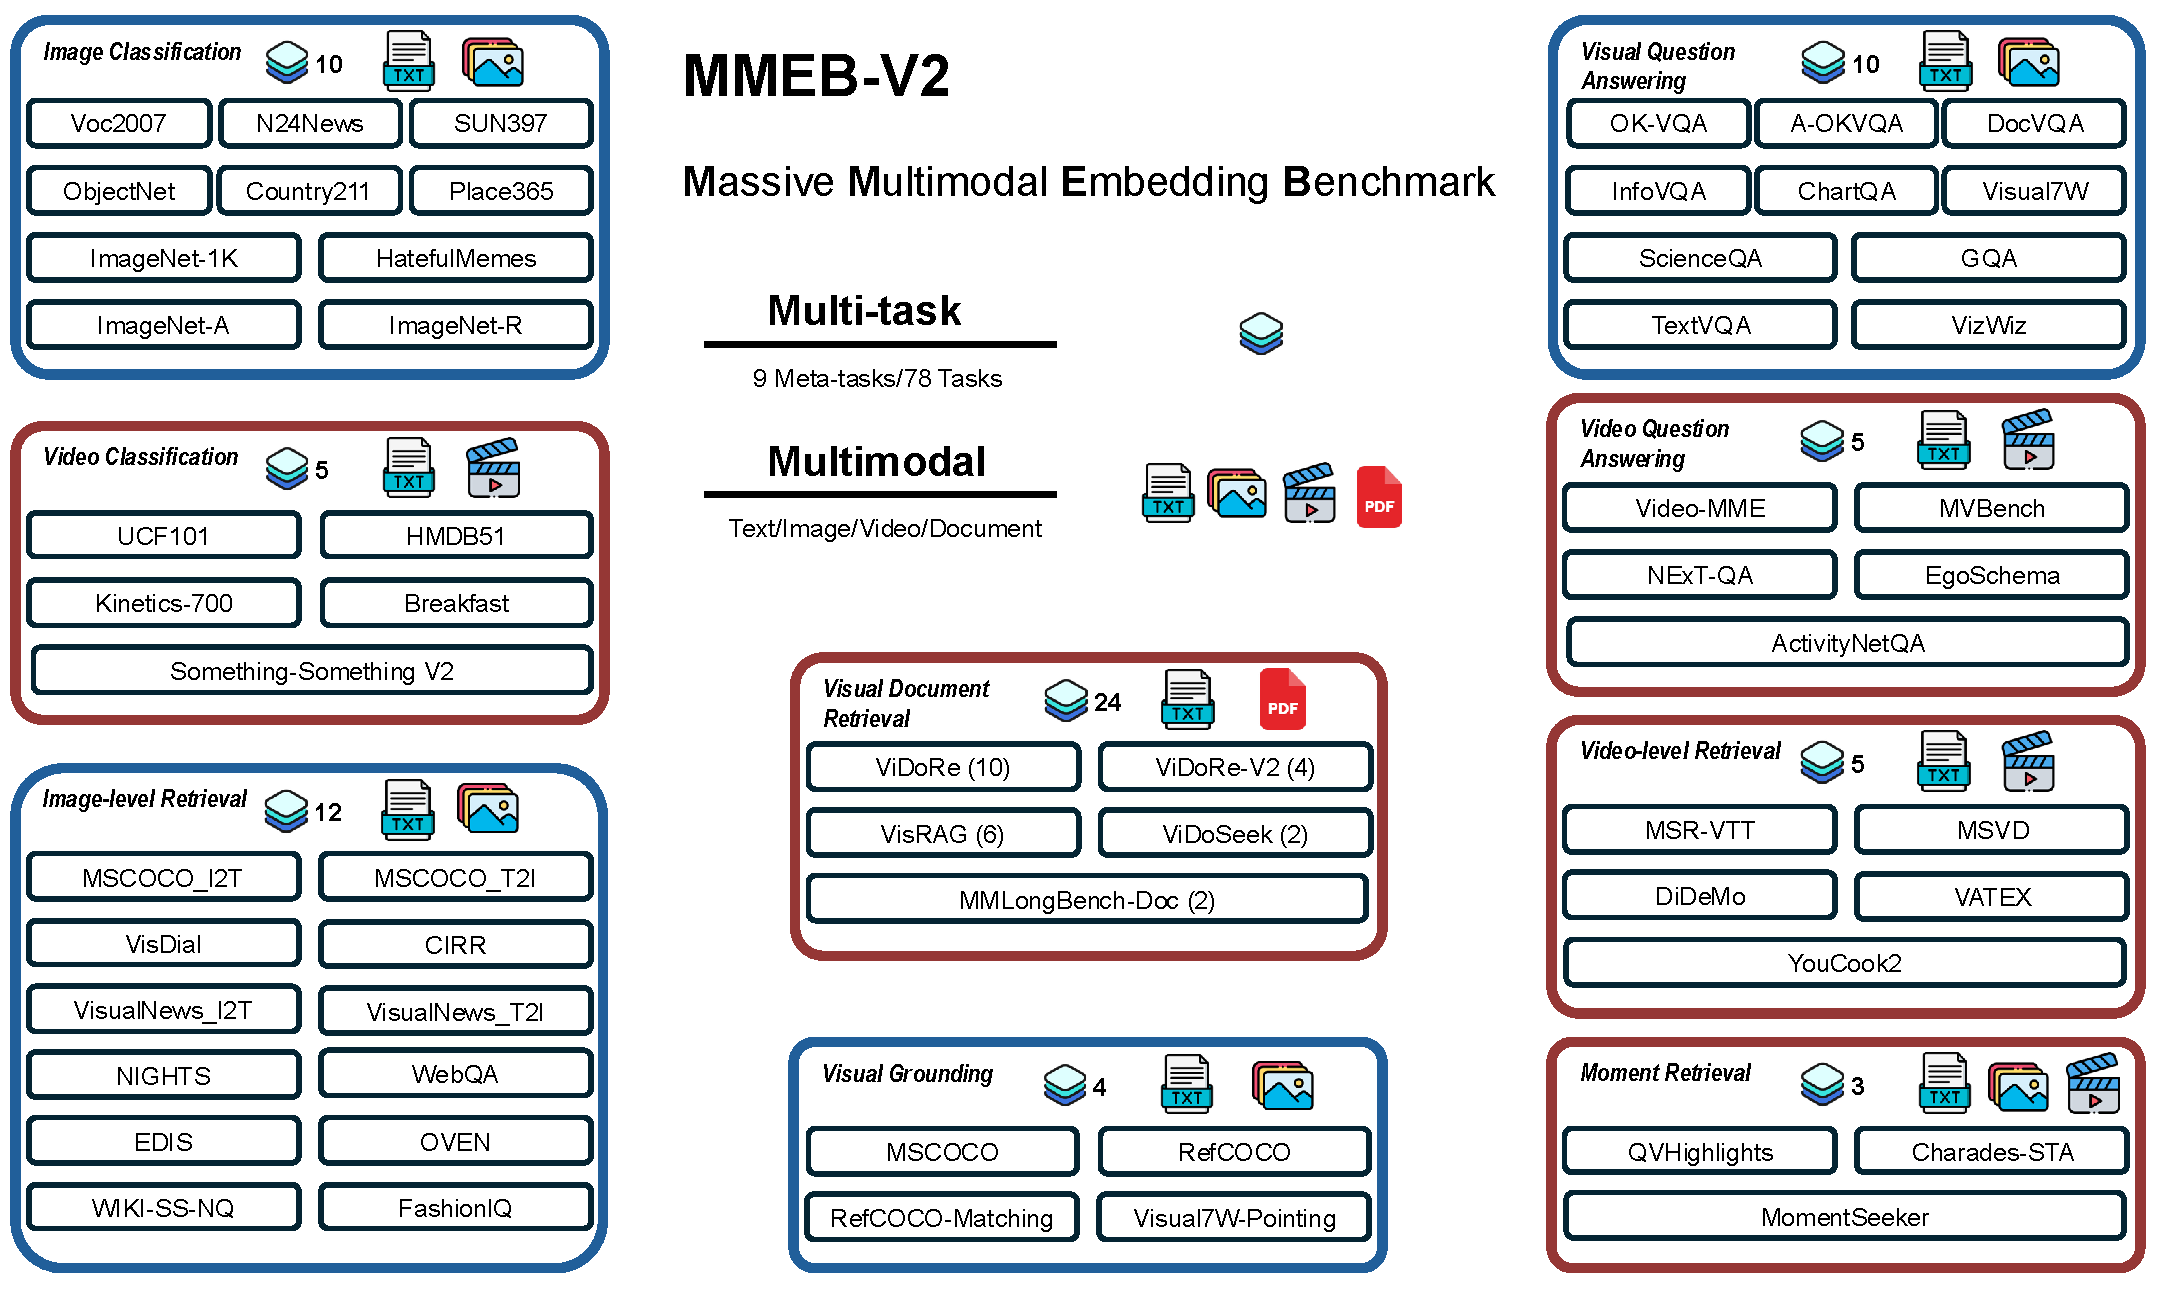
\includegraphics[width=0.9\linewidth]{figures/MMEB_V2.pdf}
    \caption{An overview of \benchmark, which includes 9 meta-tasks and 78 tasks in total. In addition to the original \mmeb benchmark, \benchmark introduces five new meta-tasks focused on video and visual documents. Tasks from \mmeb are indicated with blue borders, while newly introduced tasks in \benchmark are marked with red borders.}
    \vspace{-3ex}
    \label{fig:mmeb_pro_overview}
\end{figure}

Each task presents the model with a query and a corresponding set of candidate responses, where the goal is to select the correct target. The query consists of a combination of an instruction, a textual component, and a video or document. For video-based tasks, videos are represented as sequences of frames sampled at uniform intervals from the raw footage to ensure consistent temporal coverage. Instructions serve to specify the model's objective (e.g., ``Recognize the category of the video contents.''), and query texts can be questions, descriptions, or commands specific to the video (e.g., ``How many red socks are above the fireplace at the end of this video?'', ``Select the clips of videos that contain a dolphin.''). Each task is associated with a specific target type, which varies depending on the nature of the task. For example, in video classification, the model must identify the activity or object class label (e.g., ``Yoga'' or ``Car'').

To make the dataset practical and accessible for future research, we selectively downsample certain datasets to ensure that the full benchmark can be run within a reasonable amount of time. Our datasets span diverse domains, including sports, object recognition, daily-life activities, and movie or TV show clips. These samples are drawn from varied sources such as YouTube, professional productions, and crowd-sourced content, ensuring both diversity and real-world relevance. Summary statistics for each task are presented in Table~\ref{tab:mmeb_v2_stat}. Details about constructing each dataset are provided in Appendix~\ref{sec::appendix_baseline}.

\begin{itemize}[
    itemsep=0pt,        % remove space between items
    parsep=0pt,         % remove paragraph spacing within items
    topsep=0pt,         % remove extra space at the top
    leftmargin=1em      % adjust the left margin as needed
]
    \item \textbf{Video Retrieval (V-RET)} The query consists of an instruction, a descriptive text related to the video content, and a sequence of video frames. The model must retrieve the correct corresponding video from a pool of thousands of video candidates.
    \item \textbf{Moment Retrieval (M-RET)} The query consists of an instruction, a textual description, and optionally a full video, with the goal of retrieving the temporal segments that best matches the description. The model must select the ground-truth clip from approximately 10 candidate segments within the full video.
    \item \textbf{Video Classification (V-CLS)} Given an instruction and a sequence of video frames, the model is tasked with predicting the correct class label—related to the scene or action depicted—from a set of possible classes.
    \item \textbf{Video QA (V-QA)} The input consists of an instruction, a textual question, and a video. The model must select the correct answer from several options, including one correct choice and many distractors.
    \item \textbf{Visual Document Retrieval (VisDoc)} This task category evaluates the model’s ability to retrieve structured visual documents—such as multi-page PDFs and slide decks—in response to natural language queries. We include five datasets in this benchmark. ViDoRe V1 \& V2~\citep{colpali, vidore_v2} and VisRAG~\citep{visrag} are composed of multiple document QA datasets and cover a broad range of document types and use cases (e.g., charts and slides), though they were not originally designed for retrieval. To complement them, we include ViDoSeek~\citep{vidorag} and MMLongBench-Doc~\citep{mmlongbench}, which provide fine-grained, page-level annotations suitable for retrieval evaluation. Besides, we reformat the two datasets to support both document-level and page-level evaluation.
\end{itemize}

\begin{table}[!t]
\small
\centering
\resizebox{.9\textwidth}{!}{
\begin{tabular}{lccccc}
\toprule
\textbf{Task} & \textbf{Query MOD} & \textbf{Target MOD} & \textbf{Domain} & \textbf{\#Query} & \textbf{\#Candidates} \\
\midrule
\rowcolor{white} \multicolumn{6}{c}{\textbf{Video Retrieval (5 Tasks)}} \\
\midrule
\rowcolor{lightgray}
DiDeMo          & T     & V       & Open       & 1,004      &       1,004 \\
MSR-VTT         & T     & V       & Open       & 1,000      &       1,000 \\
\rowcolor{lightgray}
MSVD            & T     & V       & Open       & 670        &       670   \\
VATEX           & T     & V       & Open       & 4,478      &       4,478  \\
\rowcolor{lightgray}
YouCook2        & T     & V       & Cooking    & 3,179      &       3,179  \\
\midrule



\rowcolor{white} \multicolumn{6}{c}{\textbf{Moment Retrieval (3 Tasks)}} \\
\midrule
\rowcolor{lightgray}
QVHighlights    & T + V & V       & Vlog/News  & 1,083       &       10 \\
Charades-STA     & T + V & V       & Activity   & 727       &       10 \\
\rowcolor{lightgray}
MomentSeeker    & I + V & V       & Open       & 1,800 (1,602 deduped)       &       10 \\
\midrule



\rowcolor{white} \multicolumn{6}{c}{\textbf{Video Classification (5 Tasks)}} \\
\midrule
\rowcolor{lightgray}
Kinetics-700    & V     & T       &   Open     & 1,000       &       700 \\
SSv2            & V     & T       & Human-Object Interaction& 1,000      &       174 \\
\rowcolor{lightgray}
HMDB51          & V     & T       &   Open     & 1,000       &       51 \\
UCF101          & V     & T       &   Open     & 1,000       &       101 \\
\rowcolor{lightgray}
Breakfast       & V     & T       &   Cooking  & 433       &       10 \\
\midrule



\rowcolor{white} \multicolumn{6}{c}{\textbf{Video QA (5 Tasks)}} \\
\midrule
\rowcolor{lightgray}
MVBench             & V + T   & T       &     Spatial/Temporal       & 4,000 & $3 \sim 5$ \\
Video-MME              & V + T   & T       &     Real-world       & 2,700 & 4 \\
\rowcolor{lightgray}
NExT-QA              & V + T   & T       &    Daily activity        & 8,564 & 5 \\
EgoSchema      & V + T   & T       &     Egocentric       & 500 & 5 \\
\rowcolor{lightgray}
ActivityNetQA      & V + T   & T       &     Activity       & 1000 & 2 \\
\midrule



\rowcolor{white} \multicolumn{6}{c}{\textbf{Visual Document Retrieval (24 Tasks)}} \\
\midrule
\rowcolor{lightgray}
ViDoRe (10)              & T   & D       &   Documents         & 280 - 1,646 & 70 - 999 \\
ViDoRe-V2 (4)              & T   & D       &   Documents         & 52 - 640 & 452 - 1,538 \\
VisRAG (6)   & T   & D       & Documents & 63 - 816 & 500 - 9,590 \\
\rowcolor{lightgray}
ViDoSeek (2)             & T   & D      & Documents & 1,142 & 5,349 \\
MMLongBench-Doc (2)      & T   & D   & Documents & 838 & 6,492 \\
\bottomrule
\end{tabular}
}
\caption{The statistics of \benchmark, which includes \textbf{42} tasks across five meta-task categories in addition to the original \mmeb, are summarized below. Here, we list only the additional datasets introduced beyond those in \mmeb. We consider four modalities (MOD): T (Text), I (Image), V (Video), and D (Visual Document).}
\label{tab:mmeb_v2_stat}
\end{table}
